\subsection{Entity-Relationship Schema}



\begin{figure}[htbp] 
    \centering
    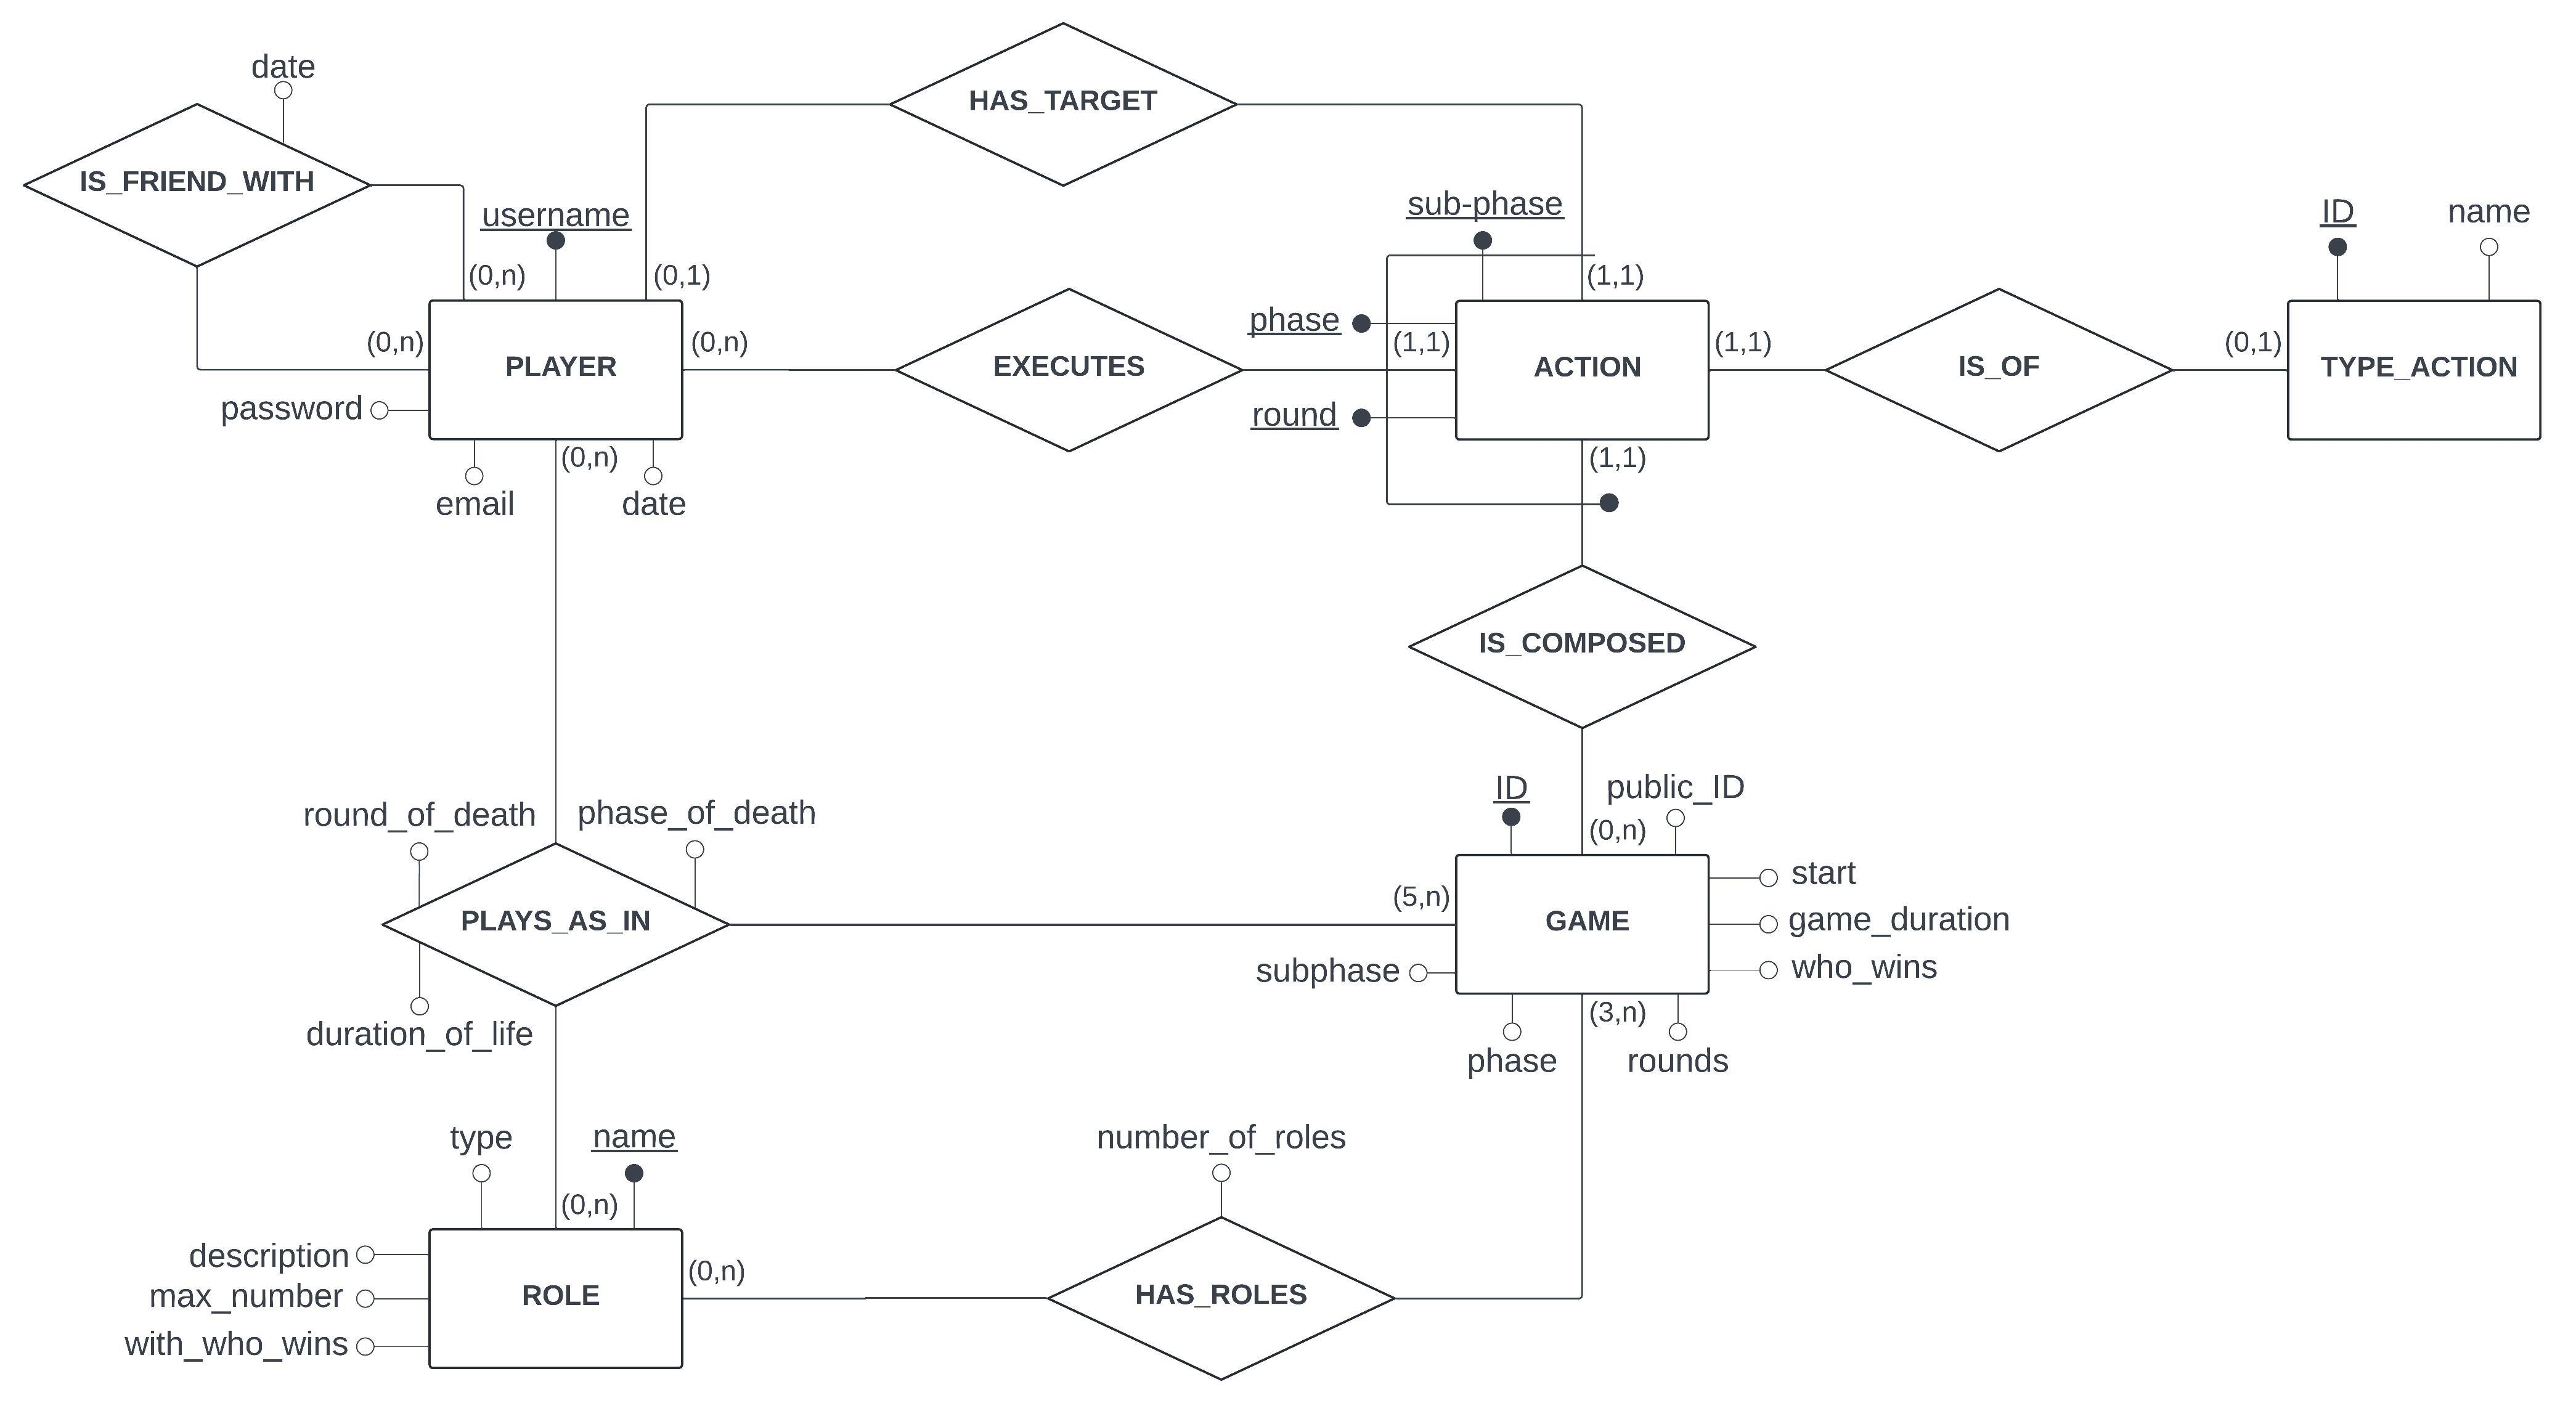
\includegraphics[width=\textwidth]{images/scheme/er_scheme_f.jpeg}
    \caption{ER scheme of LUPUS app}
    \label{fig:er_scheme}
\end{figure}

%Describe here your ER schema

The ER schema contains several entities that are:
\begin{itemize}
    \item \textbf{PLAYER}: the player entity represents the person that has subscribed to LUPUS app in order to play the game. The player creates an account providing the email and choosing a username and password. The primary key is the username (type: VARCHAR(20)) while the other attributes are email (type: VARCHAR(100), password (type: VARCHAR(100)) and date (type: DATE). The password is hashed through md5 and none attribute can be null. The email has to be unique.\\
    Each player can have a list of friends that it’s recorded in the relation called IS\_FRIEND\_WITH (containing also the attribute date (type: DATE) that indicates the date in which the player has added another player into its friends list). A player can have its friend list empty and a player does not necessarily have to be on a friends list. \\
    A player plays a specific role in a game, so is in a relation with the entities GAME and ROLE called PLAYS\_AS\_IN in which are stored the information of the duration of the life during the game. These information are contained into the attributes round\_of\_death (type: INTEGER), phase\_of\_death (type: SMALLINT, 0 for night and 1 for day) and duration\_of\_life (type: TIME).\\
    A player also can execute actions during the game so it participates in the relation EXECUTES and can be the target of an action so the player has cardinality of (0,1) with the relation HAS\_TARGET. \\
    All the other cardinality of the player are (0,n).
    \item \textbf{ROLE}: the role entity indicates the role that a player can have during the game. The role is identified by a primary key name (type: VARCHAR(20)) and has other attributes like type (type: SMALLINT), with\_who\_wins (type: SMALLINT), max\_number (type: SMALLINT) and description (type: CHARACTER VARYING). Name contains the name of the role, type indicates if the role is good, bad, neutral, victory stealer or master; with\_who\_wins indicates if the role win the game with the faction of wolves, with farmers, if it wins for itself or it's a master; max\_number contains the maximum possible number of players with the same role in a game; description contains the description of the role.\\
    Role participates in the relation PLAY\_AS\_IN and in HAS\_ROLES both with cardinality (0,n).\\
    HAS\_ROLES contains the attribute number\_of\_roles (type: SMALLINT) that indicates how much instances of a specific role are in a game. If there are no tuple of a specific role this means that the role was not present in that game.
    \item \textbf{GAME}: game is the entity that represents the match. It is identified by the primary key ID (type: SERIAL) and contains also the attributes public\_ID (type: CHARACTER VARYING), start (type: TIMESTAMP), game\_duration (type: TIME), who\_wins (type: SMALLINT), rounds (type: SMALLINT), phase (type: SMALLINT) and subphase (type: SMALLINT). public\_ID is unique and indicates public identifier of a game, it is composition of three role taken at random from the ones in the game. start and game\_duration contain the information about the start of the match  and the duration; who\_wins indicates which factions has won (farmers, wolves, hamster or jester or if the game isn't over yet); rounds represents the number of rounds played during the match; phase and subphase contain the phase and the subphase of the current game or the last phase and subphase of the game. \\
    A game is composed of several actions so participates (cardinality (0,n) into the relation IS\_COMPOSED. \\
    A game also can be played only if there are at least 5 players (cardinality (5,n) with relation PLAYS\_AS\_IN) and at least 3 roles (cardinality (3,n) with relation HAS\_ROLES). The roles needed are wolf, farmer and master.
    \item \textbf{ACTION}: action is the entity that stores all the actions that happened during a game. It is identified by a composite key formed by three identifiers one referred to the game (through the relation IS\_COMPOSED) and two to the player (through the relation EXECUTES and HAS\_TARGET) and by other three attributes: round, phase and subphase (all the types: INTEGER).\\
    The entity action participates also to another relation IS\_OF with cardinality (1,1). The relation HAS\_TARGET indicates the player that is the target of the action (can also be itself).
    \item \textbf{TYPE\_ACTION}: every action can be of a specific type like protecting, killing and seeing (the seer can ask the master if a certain person is a wolf). The type of action is identified by an ID (type: SERIAL) and there is an attribute name (type: VARCHAR(20)) containing the name of the specific type of action. A specific type of action (not the most important but maybe types of certain role) does not necessarily have to happen in a game so the cardinality with IS\_OF is (0,1). 
\end{itemize}